% The MIT License

% Copyright 2023 Shunsuke KIMURA

% Permission is hereby granted, free of charge, to any person obtaining a copy of this software and associated documentation files (the “Software”), to deal in the Software without restriction, including without limitation the rights to use, copy, modify, merge, publish, distribute, sublicense, and/or sell copies of the Software, and to permit persons to whom the Software is furnished to do so, subject to the following conditions:

% The above copyright notice and this permission notice shall be included in all copies or substantial portions of the Software.

% THE SOFTWARE IS PROVIDED “AS IS”, WITHOUT WARRANTY OF ANY KIND, EXPRESS OR IMPLIED, INCLUDING BUT NOT LIMITED TO THE WARRANTIES OF MERCHANTABILITY, FITNESS FOR A PARTICULAR PURPOSE AND NONINFRINGEMENT. IN NO EVENT SHALL THE AUTHORS OR COPYRIGHT HOLDERS BE LIABLE FOR ANY CLAIM, DAMAGES OR OTHER LIABILITY, WHETHER IN AN ACTION OF CONTRACT, TORT OR OTHERWISE, ARISING FROM, OUT OF OR IN CONNECTION WITH THE SOFTWARE OR THE USE OR OTHER DEALINGS IN THE SOFTWARE.

\documentclass[aspectratio=169,dvipdfmx,cjk]{beamer} 
\usetheme{Madrid}
\setbeamertemplate{navigation symbols}{}
\setbeamertemplate{footline}[frame number]
\usepackage{pxjahyper}
\usepackage{cite}
\usepackage{minijs}
\usepackage{listings}
\usepackage{graphicx}
\usepackage{svg}
\usepackage{xcolor}
\hypersetup{
  colorlinks=false,
  citebordercolor=green,
  linkbordercolor=red,
  urlbordercolor=cyan,
}
\lstdefinestyle{command}{
  backgroundcolor=\color{lightgray},
  basicstyle=\ttfamily\color{black},
  stringstyle={\small\ttfamily},
  keywordstyle=\color{blue},
  commentstyle=\color{gray},
  showstringspaces=false,
  frame=single,
  rulecolor=\color{lightgray},
  breaklines=true,
  numbers=left,
}
\newcommand{\cmdline}[1]{
    \colorbox{lightgray}{\lstinline[style=command]{#1}}
}
\newcommand{\blue}[1]{ {\color{blue} #1} }

\title{platex-vscode-template の使い方 \\ GUI 操作}
\author{Shunsuke Kimura}
\date{\today}

\begin{document}

\begin{frame}
  \titlepage
\end{frame}

\begin{frame}{はじめに}
  \begin{block}{概要}
    Windows を使う初学者を対象に \href{https://github.com/kimushun1101/platex-vscode-template}{https://github.com/kimushun1101/platex-vscode-template} で説明している内容のスクリーンショットを並べる.\\
    ここではとりあえず方法だけ紹介するので,気になる方は各自キーワードで検索してください.
  \end{block}
  \begin{block}{この資料でできること}
    \begin{enumerate}
      \item Windows 上にコンパイル速度が早い \LaTeX 環境の構築
      \item \LaTeX 文書作成のワークフローの習得
      \item GitHub を用いたバージョン管理および共有作業
    \end{enumerate}
  \end{block}
  \begin{tiny}
    パスワード漏洩防止や権限の適切な設定などは各人・各組織でご管理ください.
    この資料のソースコードは MIT License としています.
  \end{tiny}
\end{frame}

\begin{frame}{目次}
  \tableofcontents
\end{frame}

\begin{frame}{全体構成}
  \centering
  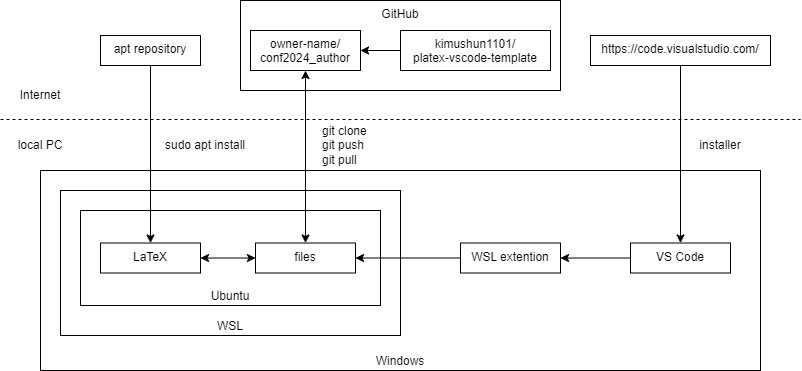
\includegraphics[width=0.9\linewidth]{fig/structure.png}
  \begin{tiny}
    \rightline{owner-name は適宜ご自身のユーザ名や組織名に置き換えてお考えください\hyperlink{create-repo}{(後述)}.}
  \end{tiny}
  多少複雑ですが,他ソースコードの編集や管理などにも流用できる技術で構成しております.
\end{frame}


\section{(初回のみ) 環境構築}

\subsection{WSL と Ubuntu のインストール}
\begin{frame}{\insertsection \thesubsection: \insertsubsection}
  Microsoft Store から Ubuntu をインストールする.
  \begin{enumerate}
    \item スタートメニューから「Store」と検索すると「Microsoft Store」が見つかる.
    \item Microsoft Store の検索窓に「Ubuntu」と検索する.
  \end{enumerate}
  \begin{columns}
    \begin{column}{0.4\textwidth}
        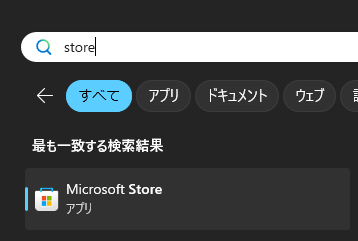
\includegraphics[width=1.0\linewidth]{fig/store.png}
    \end{column}
    \begin{column}{0.4\textwidth}
      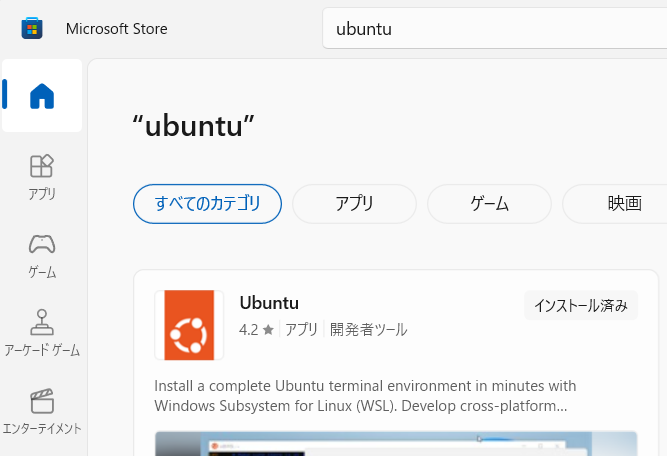
\includegraphics[width=1.0\linewidth]{fig/store-ubuntu.png}
    \end{column}
  \end{columns}
\end{frame}

\subsection{\LaTeX と Git のインストール}
\begin{frame}{\insertsection \thesubsection: \insertsubsection}
  \begin{enumerate}
    \item Ubuntu を実行.ユーザ名とパスワードを設定する.
    \item \cmdline{sudo apt update && sudo apt install texlive-full git -y} コマンドを入力.パスワードを聞かれるので設定したパスワードを入力.もしインストール中に固まってしまった場合には Enter を押せばとりあえず進む\cite{LaTeXBug}.
  \end{enumerate}
  \begin{columns}
    \begin{column}{0.3\textwidth}
        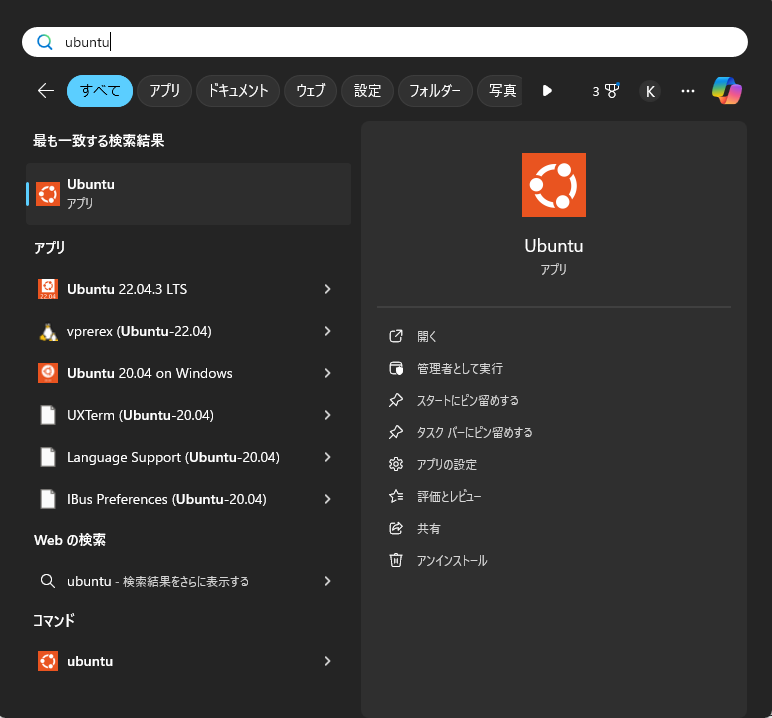
\includegraphics[width=1.0\linewidth]{fig/start-ubuntu.png}
    \end{column}
    \begin{column}{0.45\textwidth}
      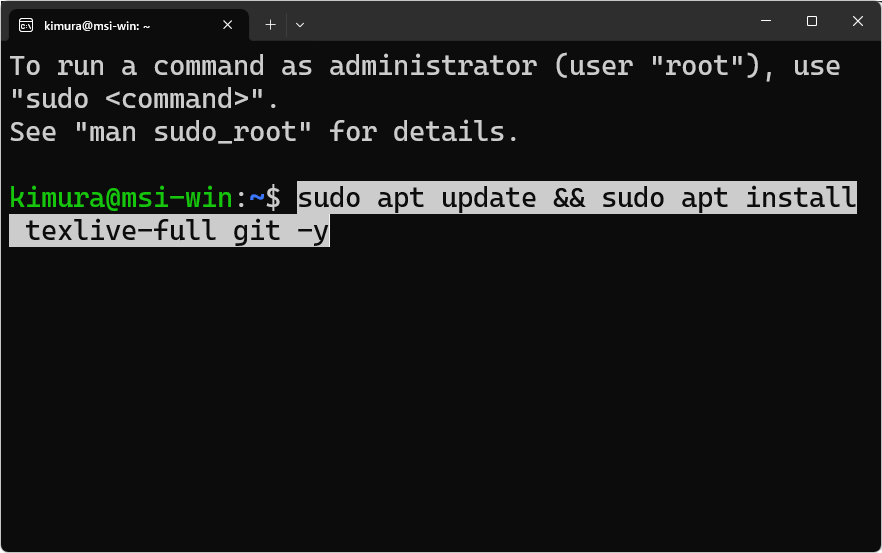
\includegraphics[width=1.0\linewidth]{fig/texlive.png}
    \end{column}
  \end{columns}
\end{frame}

\subsection{GitHub アカウントの作成}
\begin{frame}{\insertsection \thesubsection: \insertsubsection}
  \begin{enumerate}
    \item ブラウザで \href{https://github.com/}{https://github.com/} にアクセスして,\beamerbutton{Sign up for GitHub} から,ユーザ名やEメールアドレス,パスワードなどを設定\cite{GitHubAccount}.以降ログインした状態とする.
    \item GUI だけしか使わないこと前提でしたら SSH Key の登録はしなくて良いかも?\\(CLI (Command Line Interface) 版には書いています.)
  \end{enumerate}
  \begin{columns}
    \begin{column}{0.4\textwidth}
        
\includegraphics[width=1.0\linewidth]{fig/github.png}
    \end{column}
  \end{columns}
\end{frame}

\subsection{VS Code のインストール}
\begin{frame}{\insertsection \thesubsection: \insertsubsection}
  \begin{enumerate}
    \item ブラウザで\href{https://code.visualstudio.com/}{https://code.visualstudio.com/}を開き,\beamerbutton{Download for Windows} をクリックしてダウンロードできるインストーラーを実行.
    \item インストール後に VS Code を実行して \beamerbutton{Ctrl + P} で現れるテキストボックスに \cmdline{ext install ms-vscode-remote.remote-wsl} を入力して WSL Extension を install.
  \end{enumerate}
  \vspace*{5mm}
  \begin{columns}
    \begin{column}{0.33\textwidth}
        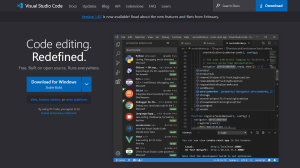
\includegraphics[width=1.0\linewidth]{fig/vscode.png}
    \end{column}
    \begin{column}{0.33\textwidth}
      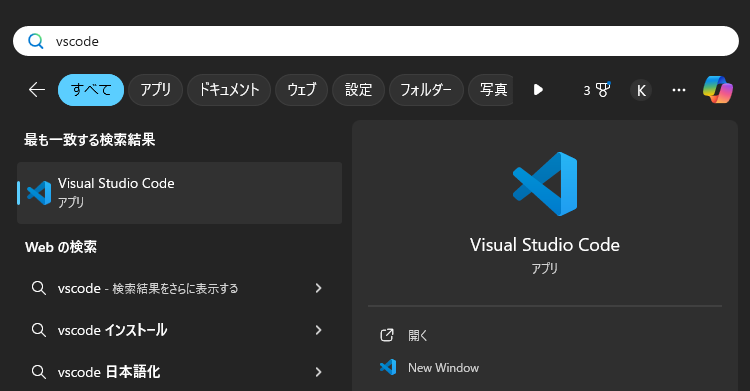
\includegraphics[width=1.0\linewidth]{fig/start-vscode.png}
    \end{column}
    \begin{column}{0.3\textwidth}
      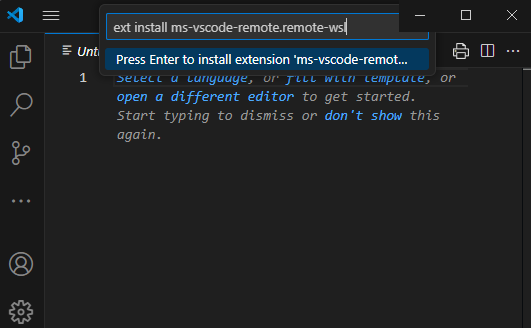
\includegraphics[width=1.0\linewidth]{fig/vscode-wsl.png}
    \end{column}
  \end{columns}
\end{frame}

\section{文書作成}
\subsection{リモート Repository の作成}
\begin{frame}[label=create-repo]{\insertsection \thesubsection: \insertsubsection}
  \begin{enumerate}
    \item \href{https://github.com/kimushun1101/platex-vscode-template}{https://github.com/kimushun1101/platex-vscode-template} にアクセス.
    \item \beamerbutton{Use this template} から \beamerbutton{create a new repository} を選択
    \item 推奨設定は以下の通り(あとから変更も可能)
    \begin{itemize}
      \item 共有したい場合には Owner を組織アカウントに変更 \hyperlink{organization}{(後述)}.
      \item Repository name は,ディレクトリ名(フォルダ名)になります.投稿先や筆頭著者名,タイトル名の一部など識別できるものを推奨.例として \cmdline{conf2024_author} としたとして進める.
      \item Private Repository にチェックを入れる.
    \end{itemize}
  \end{enumerate}
  \begin{columns}
    \begin{column}{0.4\textwidth}
        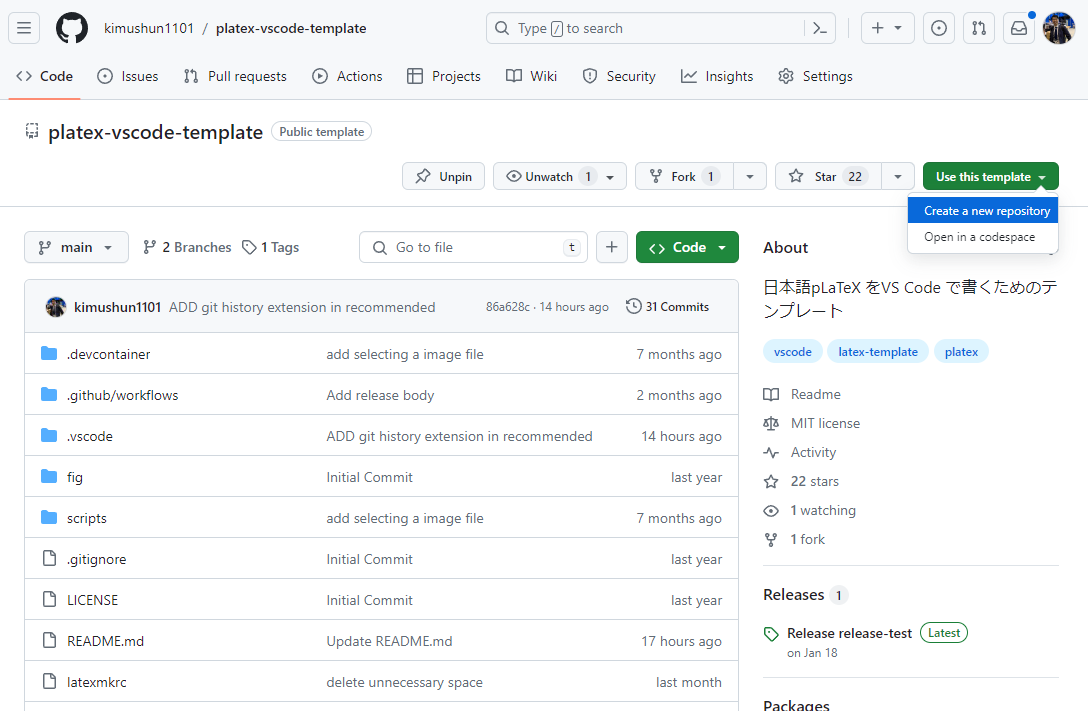
\includegraphics[width=1.0\linewidth]{fig/platex-vecode-temp.png}
    \end{column}
    \begin{column}{0.28\textwidth}
      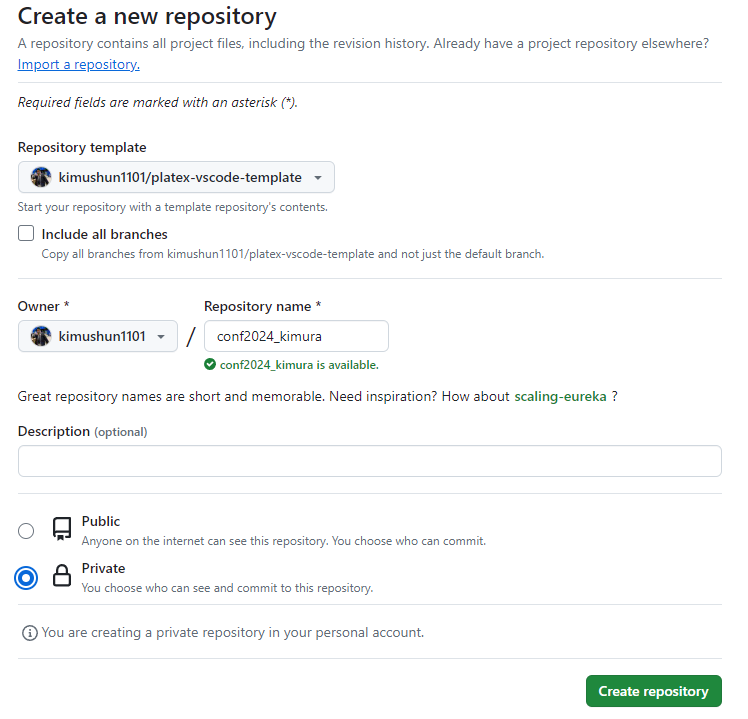
\includegraphics[width=1.0\linewidth]{fig/create-repo.png}
    \end{column}
  \end{columns}
\end{frame}

\subsection{ローカル Workspace の設定}
\begin{frame}{\insertsection \thesubsection: \insertsubsection}
  \begin{enumerate}
    \item VS Code で New Window を開く.ショートカットは \beamerbutton{Ctrl + Shif + N}.
    \item 左下の\beamerbutton{$><$} から \beamerbutton{Connect to WSL} をクリック.
    \item \beamerbutton{Clone Repository} をクリック.GitHub へのサインインを求められたら行う\cite{GitHubAuthentication}.
    \item \beamerbutton{Clone from GitHub} から今回作成した \cmdline{conf2024_author} を選択.
  \end{enumerate}
  \begin{columns}
    \begin{column}{0.25\textwidth}
        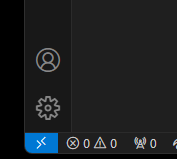
\includegraphics[width=1.0\linewidth]{fig/connect.png}
    \end{column}
    \begin{column}{0.3\textwidth}
      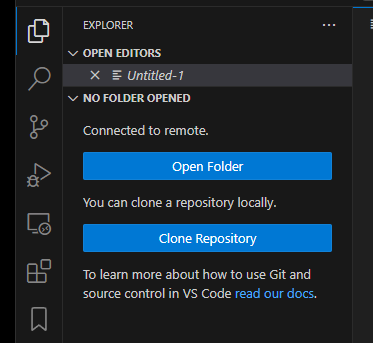
\includegraphics[width=1.0\linewidth]{fig/clone-gui.png}
    \end{column}
    \begin{column}{0.3\textwidth}
      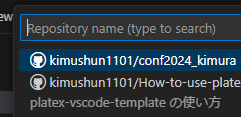
\includegraphics[width=1.0\linewidth]{fig/select-repo.png}
    \end{column}
  \end{columns}
\end{frame}

% \begin{frame}{\insertsection \thesubsection: \insertsubsection (コマンドライン)}
%   \begin{enumerate}
%     \item 前スライドで作成したRepositoryのページを開く.
%     \href{https://github.com/}{https://github.com/} から探せる.
%     \item \beamerbutton{$< >$ Code▼} から \beamerbutton{SSH} タブを選択,\beamerbutton{□が2つ重なったような記号} をクリックして URL をコピー.
%     \item Ubuntu に \cmdline{git clone URL} コマンドを\blue{コピーしたURLに置き換えて}入力.\\
%     Are you sure you want to continue connecting? には \cmdline{yes} と答える.
%     \item Ubuntu に \cmdline{code conf2024_author} コマンドを\blue{自身のrepository名に置き換えて}入力することで,VS Code を起動する.\beamerbutton{Yes, I trust the authors} をクリック.
%     \begin{itemize}
%       \item \cmdline{ls} コマンドをすると現在存在するディレクトリを確認できる.興味があれば「Unix コマンド」で調べてみるとよい.移動や削除など,よりいろいろな操作ができるようになるだろう.
%       \item たとえば \cmdline{code conf[Tab]} という感じで,途中まで入力してTab キーで補完もできる.
%     \end{itemize}
%   \end{enumerate}
%   \begin{columns}
%     \begin{column}{0.25\textwidth}
%         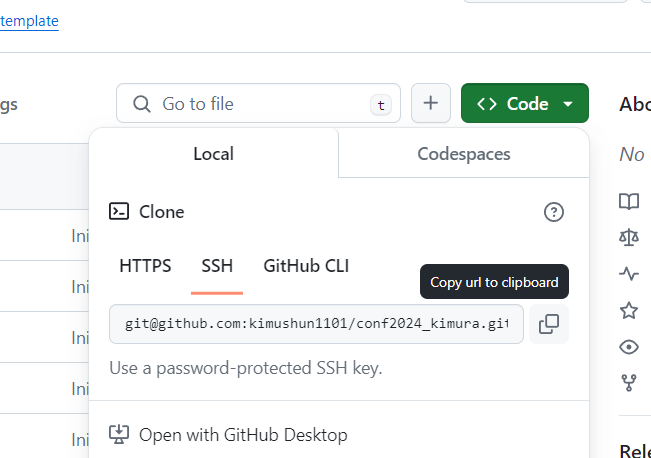
\includegraphics[width=1.0\linewidth]{fig/clone-url.png}
%     \end{column}
%     \begin{column}{0.3\textwidth}
%       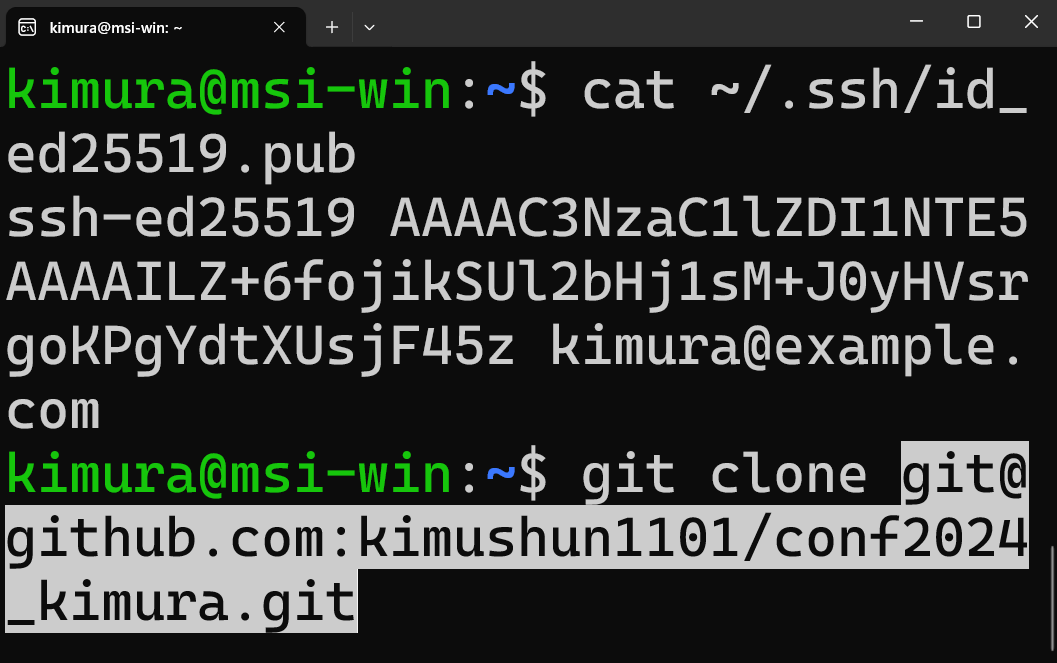
\includegraphics[width=1.0\linewidth]{fig/git-clone.png}
%     \end{column}
%     \begin{column}{0.3\textwidth}
%       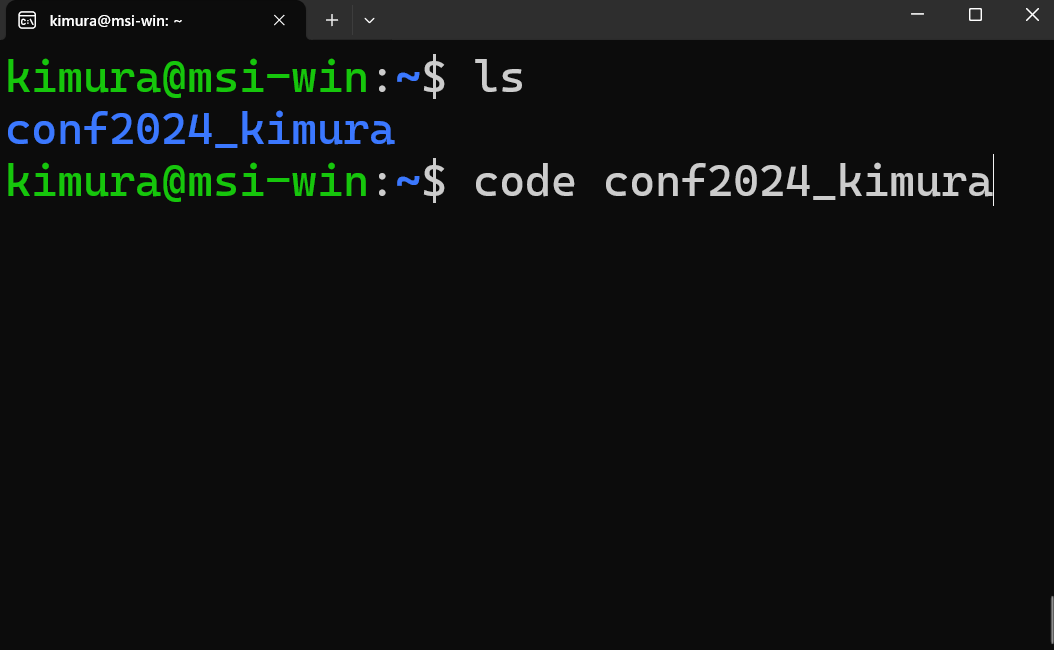
\includegraphics[width=1.0\linewidth]{fig/code-repo.png}
%     \end{column}
%   \end{columns}
% \end{frame}

\subsection{(初回のみ) VS Code 拡張機能のインストール}
\begin{frame}{\insertsection \thesubsection: \insertsubsection}
  \begin{enumerate}
    \item VS Code 画面左にある Extensions を開く.ショートカットは \beamerbutton{Ctrl + Shif + X}.
    \item 検索ボックス右の Filter Extensions をクリックして,\beamerbutton{recommended} を選択して出てきたものをすべてインストールする.
  \end{enumerate}
  \begin{columns}
    \begin{column}{0.45\textwidth}
        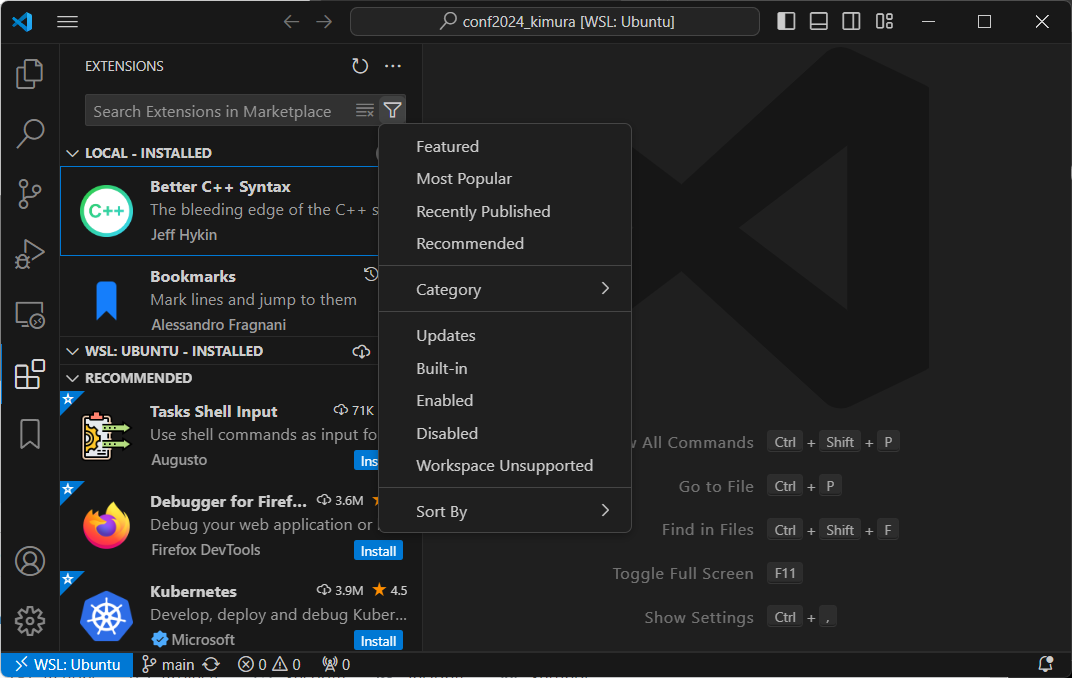
\includegraphics[width=1.0\linewidth]{fig/vscode-extentions.png}
    \end{column}
    \begin{column}{0.45\textwidth}
      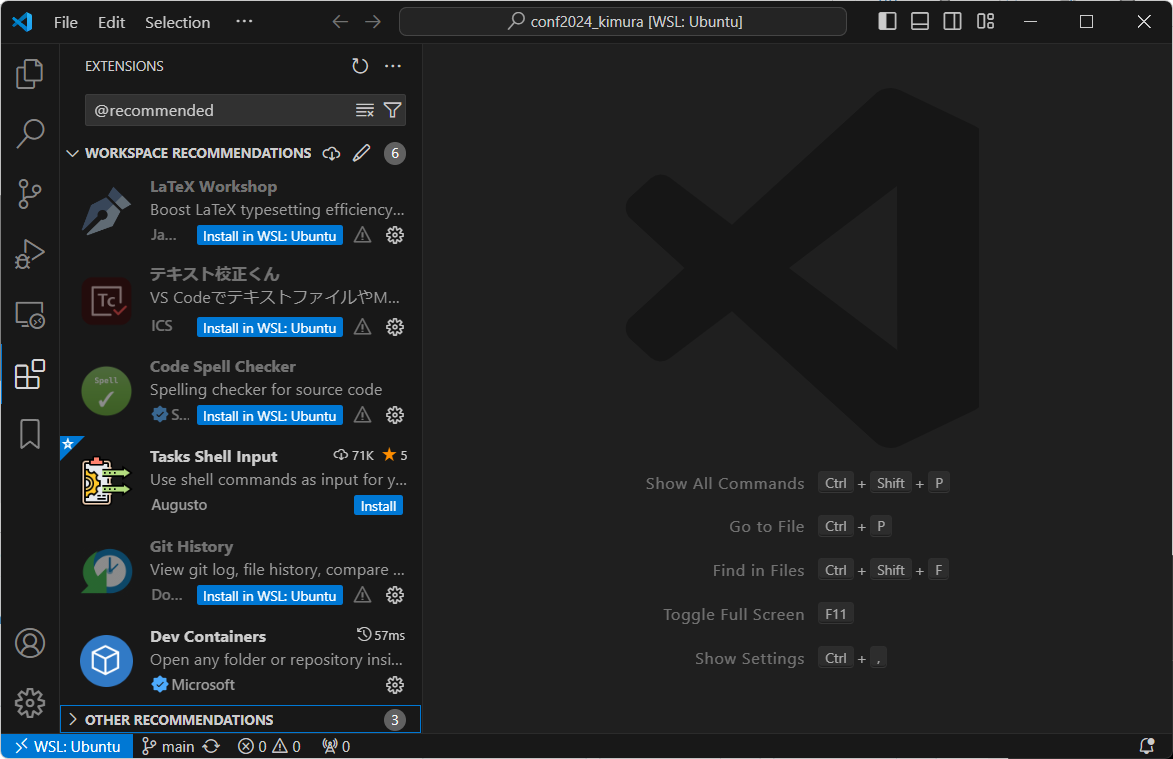
\includegraphics[width=1.0\linewidth]{fig/vscode-recommneded.png}
    \end{column}
  \end{columns}
\end{frame}

\subsection{編集作業}
\begin{frame}{\insertsection \thesubsection: \insertsubsection (サンプルの確認)}
  \begin{enumerate}
    \item VS Code 画面左にある Explore を開く.ショートカットキーは \beamerbutton{Ctrl + Shift + E}.
    \item sample.tex をクリックして開く.
    \item \beamerbutton{Ctrl + Alt + B} でビルド.ファイル保存時もオートビルドされる.
    \item \beamerbutton{Ctrl + Alt + V} でコンパイル済みPDFを表示.
  \end{enumerate}
  その他のショートカットは以下の通り.\\
  \vspace{10mm}
  \centering
  \begin{tabular}{ll} \hline
    ショートカット & 機能 \\
    \hline
    \beamerbutton{Ctrl + Alt + J} & PDF の該当の場所にジャンプ \\
    PDF を \beamerbutton{Ctrl} + クリック & .tex の該当の行にジャンプ \\
    \beamerbutton{Ctrl + Alt + M} & 数式プレビューの表示 \\
    \beamerbutton{Ctrl + J} (PROBLEMS タブ) & エラーやワーニングの確認 \\
    \beamerbutton{F8} & エラーやワーニングへジャンプ \\
    \hline
  \end{tabular}
\end{frame}

\begin{frame}{\insertsection \thesubsection: \insertsubsection (テンプレートの導入)}
  \begin{enumerate}
    \item 学会などから投稿先のテンプレートファイルを入手.圧縮されている場合は展開する.
    \item \beamerbutton{Ctrl + Shift + P} から \cmdline{Tasks: Run Task} を選択し,つづけて\cmdline{Open the workspace with explore} を選択.フォルダにファイルをコピーする.
    \item ビルドしたい .tex ファイルを開きビルドする.ファイル名はsample.tex でなくても有効.
  \end{enumerate}
  \begin{columns}
    \begin{column}{0.45\textwidth}
        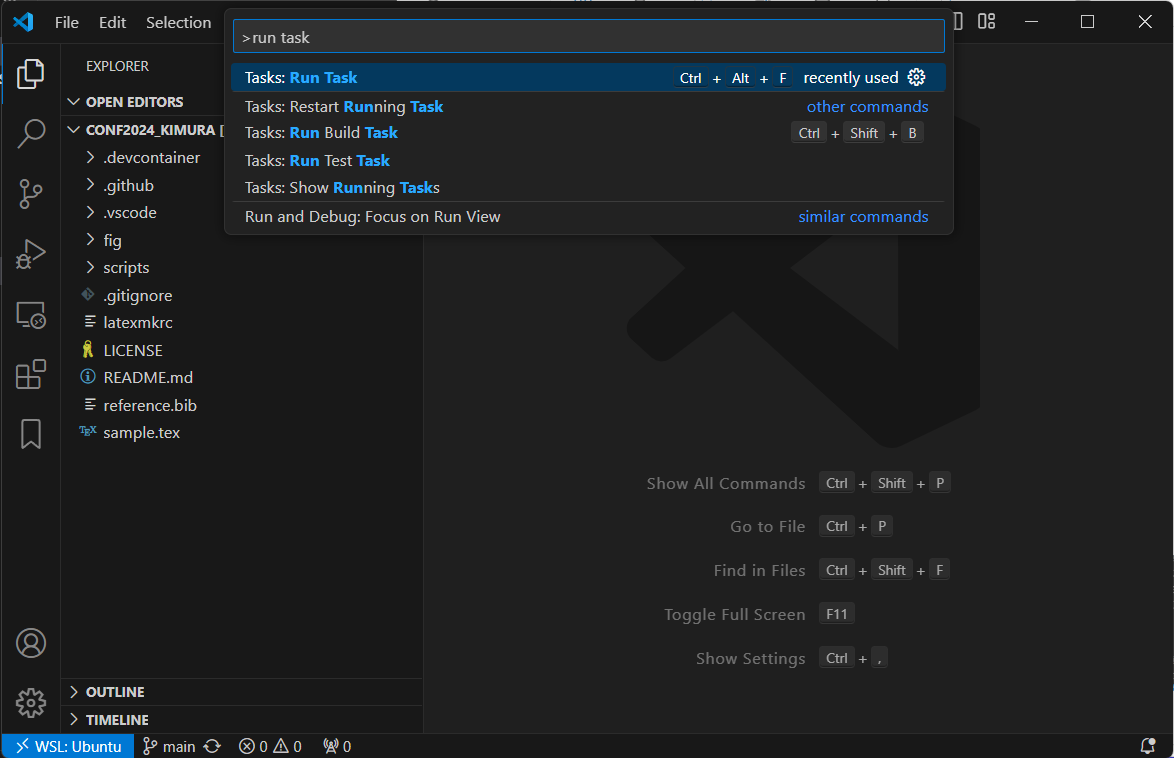
\includegraphics[width=1.0\linewidth]{fig/run-task.png}
    \end{column}
    \begin{column}{0.45\textwidth}
      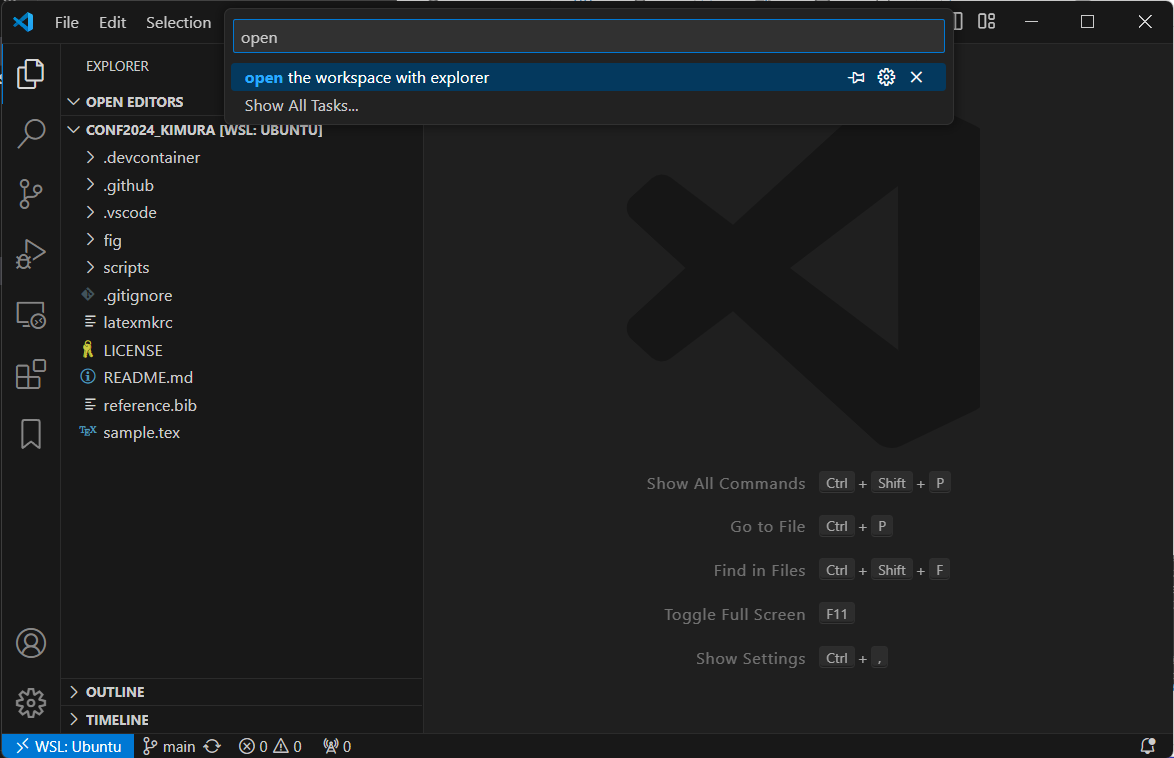
\includegraphics[width=1.0\linewidth]{fig/open-workspace.png}
    \end{column}
  \end{columns}
\end{frame}

\subsection{バージョンの保存}
\begin{frame}[label=git]{\insertsection \thesubsection: \insertsubsection}
  \begin{enumerate}
    \item VS Code 画面左にある Source Control を開く.ショートカットキーは \beamerbutton{Ctrl + Shift + G}.
    \item Changes から保存したいファイルを\beamerbutton{+}で追加.Staged Changes に乗せる.
    \item Message に今回の変更内容を記入.
    \item \beamerbutton{Commit} の後,\beamerbutton{Sync Changes} でアップロード.
    \item ブラウザで GitHub repository ページを更新するとアップロードを確認できる.
  \end{enumerate}
  \begin{columns}
    \begin{column}{0.3\textwidth}
        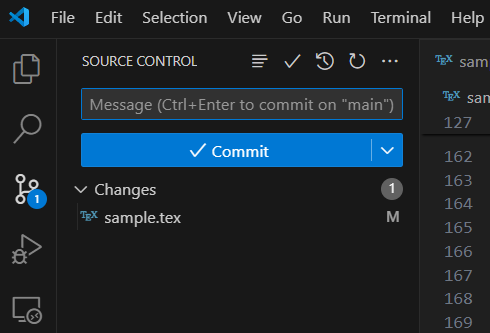
\includegraphics[width=1.0\linewidth]{fig/git-control.png}
    \end{column}
    \begin{column}{0.3\textwidth}
      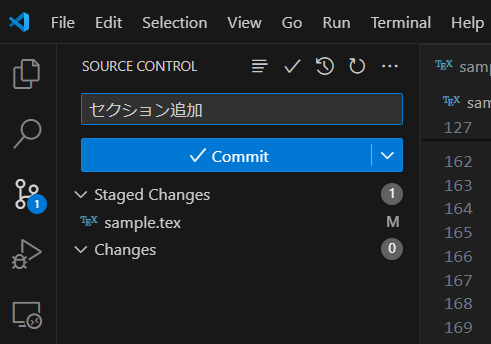
\includegraphics[width=1.0\linewidth]{fig/git-commit.png}
    \end{column}
    \begin{column}{0.3\textwidth}
      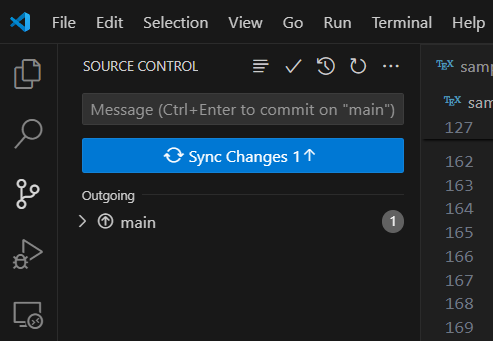
\includegraphics[width=1.0\linewidth]{fig/git-sync.png}
    \end{column}
  \end{columns}
\end{frame}

\section{共同作業}
\subsection{(初回のみ) 組織アカウントの作成}
\begin{frame}[label=organization]{\insertsection \thesubsection: \insertsubsection}
  組織アカウントが Owner である Private Repository は,組織アカウントに紐づけられた個人アカウントのみ閲覧することができる.
  \begin{enumerate}
    \item \href{https://github.com/}{https://github.com/} の左上にある \beamerbutton{+} から \beamerbutton{New organization} をクリック.
    \item とりあえずは Free プランの \beamerbutton{Create a free organization} を選択する.
    \item Organization name や Eメールアドレスなどを入力して作成.
    \item \href{https://github.com/organization-name}{https://github.com/organization-name} を\blue{organization-nameを置き換えて}アクセス.
    \item People タブから \beamerbutton{Invite member} をクリックして,メンバーを追加.
  \end{enumerate}
  \begin{columns}
    \begin{column}{0.3\textwidth}
        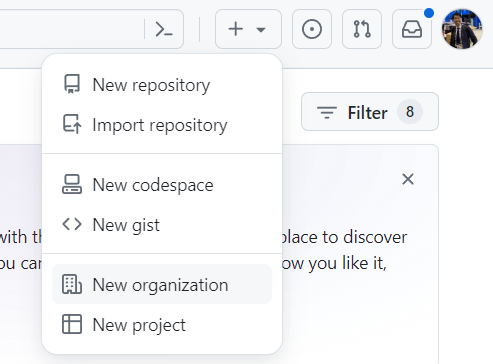
\includegraphics[width=1.0\linewidth]{fig/new-organization.png}
    \end{column}
    \begin{column}{0.6\textwidth}
      
\includegraphics[width=1.0\linewidth]{fig/invite-member.png}
    \end{column}
  \end{columns}
\end{frame}

\subsection{変更箇所の確認}
\begin{frame}{\insertsection \thesubsection: \insertsubsection}
  \begin{enumerate}
    \item Source Control から \beamerbutton{Sync Changes} で,他の人が行った変更を取り込む.
    \item VS Code で Explore を開く.ショートカットキーは \beamerbutton{Ctrl + Shift + E}.
    \item 履歴をみたいファイルを右クリックして\beamerbutton{Git: View file history} を選択.ショートカットは \beamerbutton{Alt + H}.
    \item 対象のコミットを選択して,対象のファイルの \beamerbutton{Workspace} をクリック.
    \item 対象のファイルの \beamerbutton{View} をクリックすれば,そのコミット時点での内容を確認できる.
  \end{enumerate}
  \begin{columns}
    \begin{column}{0.3\textwidth}
        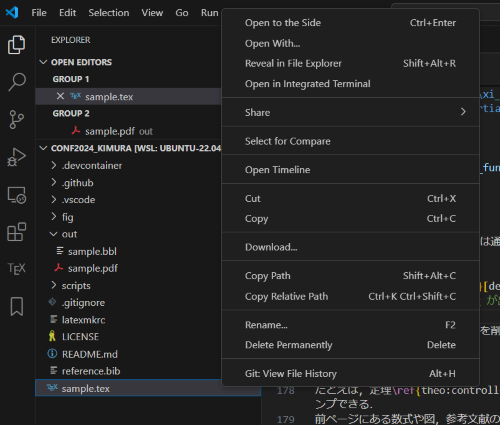
\includegraphics[width=1.0\linewidth]{fig/git-history1.png}
    \end{column}
    \begin{column}{0.3\textwidth}
      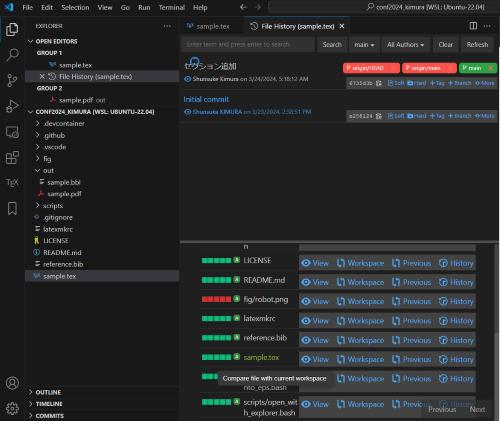
\includegraphics[width=1.0\linewidth]{fig/git-history2.png}
    \end{column}
    \begin{column}{0.3\textwidth}
      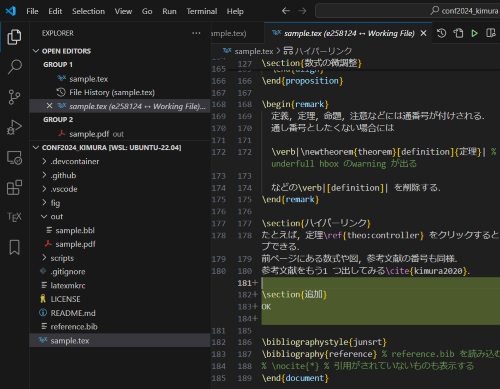
\includegraphics[width=1.0\linewidth]{fig/git-history3.png}
    \end{column}
  \end{columns}
\end{frame}

\subsection{コンフリクト(競合)の解消}
\begin{frame}{\insertsection \thesubsection: \insertsubsection}
  自身の変更をアップロードする前に,他の人の変更がアップロードされていた場合,手元でコンフリクトを解決したコミットを作成してからアップロードする.
  \begin{enumerate}
    \item \hyperlink{git}{バージョンの保存} をした際にポップアップが出た場合,\\
    \beamerbutton{Sync Changes} がダウンロード・アップロード両方ある状態であることが確認できる.
    \item SOURCE CONTROL の \beamerbutton{$\cdots$} から \beamerbutton{Branch},\beamerbutton{Marge} をクリックし,\beamerbutton{origin/main} を選択.
    \item \beamerbutton{Accept Current Change} や \beamerbutton{Accept Incoming Change} などをクリックして,適宜追加変更する.
    \item 編集したファイルを\beamerbutton{+}で追加,\beamerbutton{Commit} の後,\beamerbutton{Sync Changes} でアップロード.
  \end{enumerate}
  \begin{columns}
    \begin{column}{0.23\textwidth}
        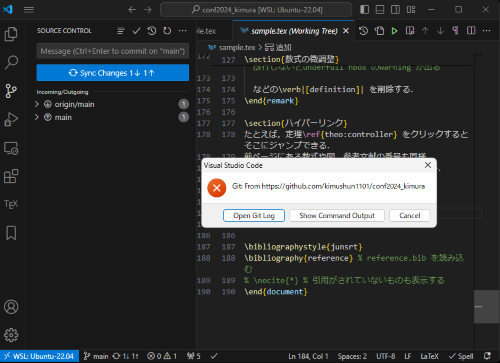
\includegraphics[width=1.0\linewidth]{fig/git-conflict.png}
    \end{column}
    \begin{column}{0.23\textwidth}
      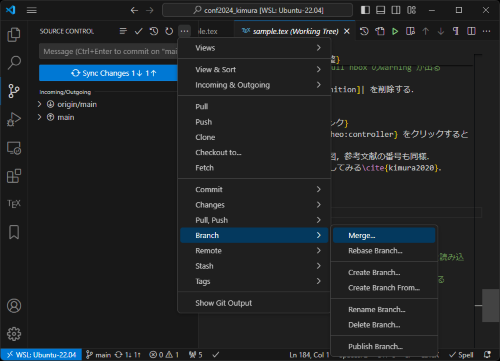
\includegraphics[width=1.0\linewidth]{fig/git-marge.png}
    \end{column}
    \begin{column}{0.23\textwidth}
      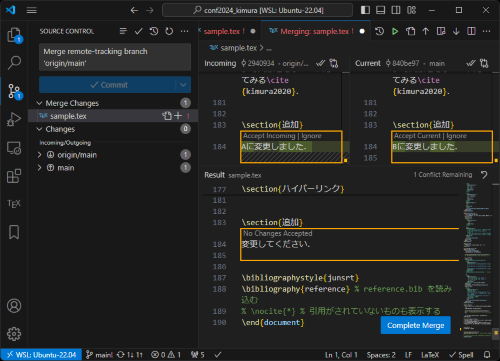
\includegraphics[width=1.0\linewidth]{fig/git-editor.png}
    \end{column}
    \begin{column}{0.23\textwidth}
      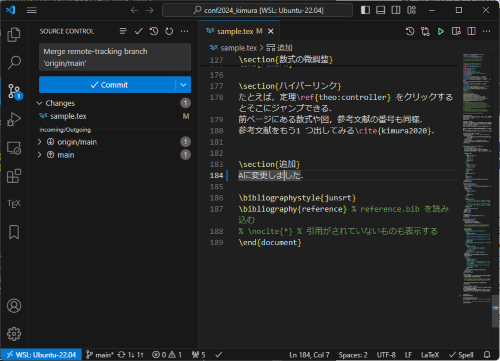
\includegraphics[width=1.0\linewidth]{fig/git-solve-conflict.png}
    \end{column}
  \end{columns}
\end{frame}

\section*{参考URL}
\begin{frame}{\insertsection}
  \scriptsize
  \begin{thebibliography}{99}
  \beamertemplatetextbibitems

  % \bibitem{WSL} WSL を使用して Windows に Linux をインストールする方法\\
  % \href{https://learn.microsoft.com/ja-jp/windows/wsl/install}{https://learn.microsoft.com/ja-jp/windows/wsl/install}

  \bibitem{LaTeXBug} Pregenerating ConTeXt MarkIV format. This may take some time... takes forever\\
  \href{https://askubuntu.com/questions/956006/pregenerating-context-markiv-format-this-may-take-some-time-takes-forever
  }{https://askubuntu.com/questions/956006/pregenerating-context-markiv-format-this-may-take-some-time-takes-forever}

  \bibitem{GitBook} Git Book 1.6 Getting Started - First-Time Git Setup\\
  \href{https://git-scm.com/book/en/v2/Getting-Started-First-Time-Git-Setup
  }{https://git-scm.com/book/en/v2/Getting-Started-First-Time-Git-Setup}

  \bibitem{GitHubAccount} GitHub アカウントの概要\\
  \href{https://docs.github.com/ja/get-started/onboarding/getting-started-with-your-github-account
  }{https://docs.github.com/ja/get-started/onboarding/getting-started-with-your-github-account}
  
  % \bibitem{GitHubSSH} GitHub アカウントへの新しい SSH キーの追加\\
  % \href{https://docs.github.com/ja/authentication/connecting-to-github-with-ssh/adding-a-new-ssh-key-to-your-github-account
  % }{https://docs.github.com/ja/authentication/connecting-to-github-with-ssh/adding-a-new-ssh-key-to-your-github-account}

  \bibitem{GitHubAuthentication} GitHub への認証方法について\\
  \href{https://docs.github.com/ja/authentication/keeping-your-account-and-data-secure/about-authentication-to-github
  }{https://docs.github.com/ja/authentication/keeping-your-account-and-data-secure/about-authentication-to-github}

  % \bibitem{GitStash} Git Book 7.3 Git Tools - Stashing and Cleaning\\
  % \href{https://git-scm.com/book/en/v2/Git-Tools-Stashing-and-Cleaning
  % }{https://git-scm.com/book/en/v2/Git-Tools-Stashing-and-Cleaning}

  \end{thebibliography}
\end{frame}

\end{document}